\documentclass[12pt,letterpaper,notitlepage,openany]{article}

\usepackage[margin=1in]{geometry}
\usepackage{graphicx}
\usepackage[square,numbers]{natbib}
\usepackage[titles]{tocloft}
\usepackage{amsmath}
\usepackage{amssymb}
\usepackage{epstopdf}
\usepackage{dcolumn}% Align table columns on decimal point
\usepackage{bm}% bold math
\usepackage{setspace}
\usepackage{rotating}
%\usepackage{csvsimple}
\usepackage[caption=false,font=footnotesize]{subfig}
\usepackage{fixltx2e}
\usepackage{placeins}
\usepackage{textcomp}

\newcommand*{\etal}{\emph{et al.}~}

% of the American Astronomical Society.
%\usepackage{deluxetable}		% Allows use of AASTEX deluxe tables
%\usepackage{aastex_hack}		% Allows other AASTEX functionality.

% These are other packages that you might find useful.
% For controlling the fonts, see
% http://www.math.uiuc.edu/~hartke/computer/latex/survey/survey.html
% The following is a nice font set:
%\usepackage{mathtime}			% Times for letters; Belleek math.
%
%\usepackage{lscape}			% Used for making fitting large tables in by putting them landscape
%\usepackage{refs}
%
% If you are using hyper-ref (recommended), this command must go after all
% other package inclusions (from the hyperref package documentation).
% The purpose of hyperref is to make the PDF created extensively
% cross-referenced.
\usepackage[pdftex,bookmarks,colorlinks=true,urlcolor=black,linkcolor=black,citecolor=black]{hyperref}
\usepackage[capitalise]{cleveref}

\begin{document}
\title{DISSERTATION PROPOSAL:\\ DESIGN AND USE OF AN IRRADIANCE
  MONITORING NETWORK FOR SHORT-TERM IRRADIANCE FORECASTING}
\author{Antonio T. Lorenzo}
\date{Feb. 22, 2017}
\maketitle

\begin{abstract}
  Short-term solar irradiance forecasts help electric utilities add
  more solar power plants while maintaining a reliable grid. This
  dissertation studies new methods to produce short-term forecasts
  that rely on an irradiance monitoring network. As part of this
  forecasting effort, we designed and deployed inexpensive irradiance
  sensors in Tucson, AZ. These sensors, along with data from rooftop
  PV systems, are used to produce irradiance forecasts for 1 min to 60
  min in the future. For longer time horizons (30 min to 4 h),
  forecasts produced from satellite images are used. We have improved
  the irradiance estimates of individual satellite images by combining
  the satellite estimate and data from the sensor network. These
  improved satellite derived nowcasts will be the basis of future work
  that will continuously assimilate data into satellite derived
  forecasts.
\end{abstract}

\section{Introduction}
Solar power forecasts help control the costs associated with the
intermittency of solar power \citep{Joskow2011} by, for example,
enabling smarter control of battery storage to control ramp-rates and
provide frequency support \citep{Hill2012,Cormode2015} or more
efficiently scheduling generators.
Since global horizontal irradiance (GHI) is the primary driver of
non-concentrating solar power production, forecasting techniques often
first forecast GHI and then produce a power forecast
\citep{Kleissl2013,Inman2013}.
For forecast horizons from a few seconds to a few minutes, statistical
techniques applied to data from ground sensors are often used
\citep{Yang2015,Lipperheide2015}.
Intra-hour forecasts may use a sensor network \citep{Lonij2013},
machine learning techniques \citep{Chu2013}, or sky cameras
\citep{Chow2011}.
Forecasts based on satellite images are used for time horizons from
roughly 1 h to 6 h in advance \citep{Perez2010}, while numerical
weather predictions are used for forecasts horizons extending from
many hours to many days in advance \citep{Perez2013}.


The goal of this dissertation is to study, in depth, short-term
forecasting techniques that rely on data from a sensor network.
First, we describe the sensor network that we built in Tucson, AZ, for
this purpose.
Then, we describe forecasts for 1 min to 1 h in advance using only
data from this network \citep{Lorenzo2015c}.
We studied forecast errors in depth as part of this work to understand
that simple error metrics may not be enough to determine which
forecasting method is ``best.''
For longer time horizon forecasts, which require estimates of
irradiance over a larger area, irradiance derived from satellite
images is an ideal starting point.
One problem is that the initial satellite estimate, or nowcast, often
has large errors when compared to ground measurements.
Utilizing the network data and a method known as optimal interpolation
(OI) we improved these satellite nowcasts to more closely resemble
reality \citep{Lorenzo2017}.
Future work (by other students) will focus on extending OI with a
cloud advection scheme to continuously assimilate new ground and
satellite data, and to combine the forecasts that are made for
different time horizons into a single, unified forecast.
A summary of the errors for methods studied in this dissertation is
presented in \cref{fig:bullshitplot}.

\begin{figure}[h]
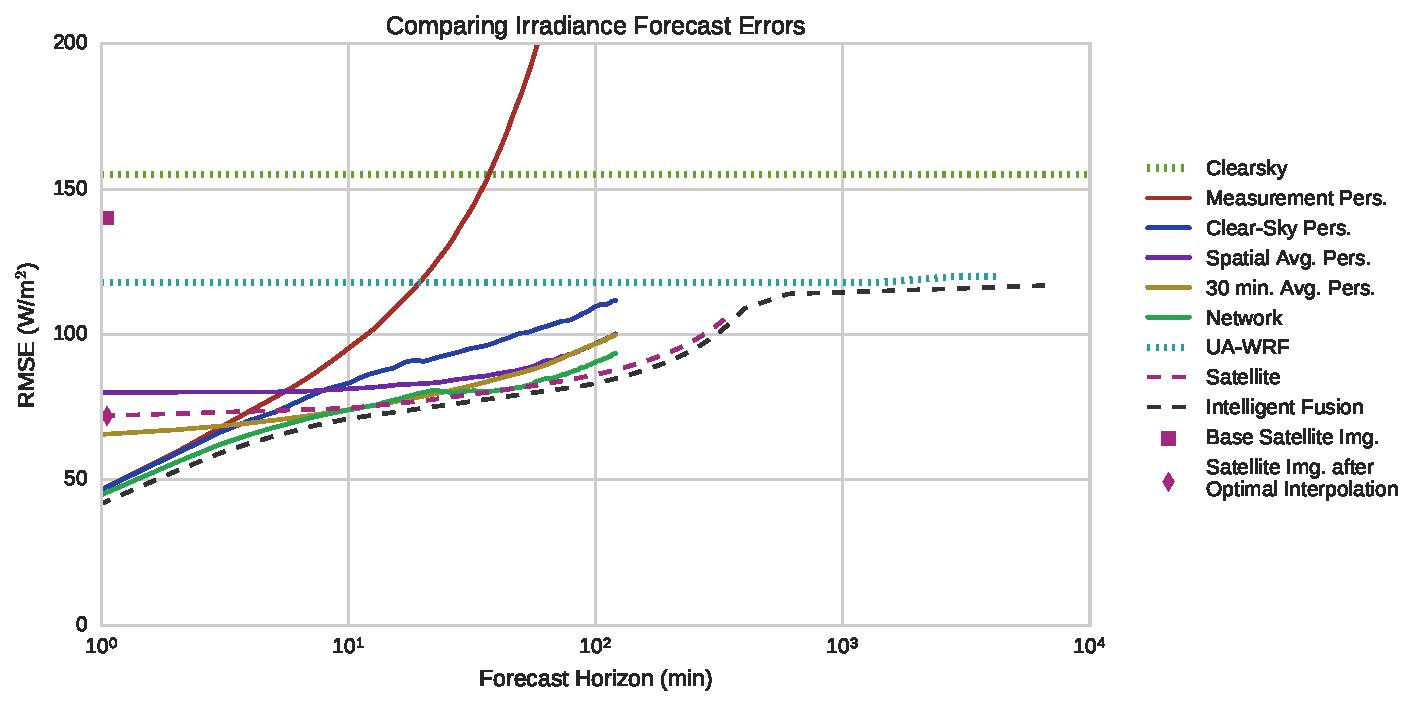
\includegraphics[width=\textwidth]{../dissertation/figs/timehorizon.pdf}
\caption[Irradiance forecast errors across forecast horizons]{A
  comparison of irradiance forecast root-mean squared errors (RMSE)
  across many time horizons. The solid lines (and points) indicate
  forecasts that will be studied in depth in this dissertation. Dashed
  lines are based on prelimnary analysis, but have not been studied in
  depth. Pers.\ refers to persistence, and UA-WRF refers to the
  numerical weather models generated at the UA using the Weather
  Research and Forecasting (WRF) model. The intelligent fusion is a
  theoretical combination of forecasts at diffferent time horizons for
  the best forecast at all horizons.}
\label{fig:bullshitplot}
\end{figure}


\section{Irradiance Monitoring Network}
Lonij \etal described forecasts made using an network of rooftop PV
systems as sensors \citep{Lonij2013}.
To extend and to provide this type of forecast to utilities
operationally, we built an irradiance montioring network with the
primary goal of receiving data in real-time and with sufficient
density to produce accurate forecasts.
This led to the construction of the irradiance monitoring network.

\begin{figure}[ht]
\centering
\captionsetup[subfigure]{labelformat=empty}
\subfloat{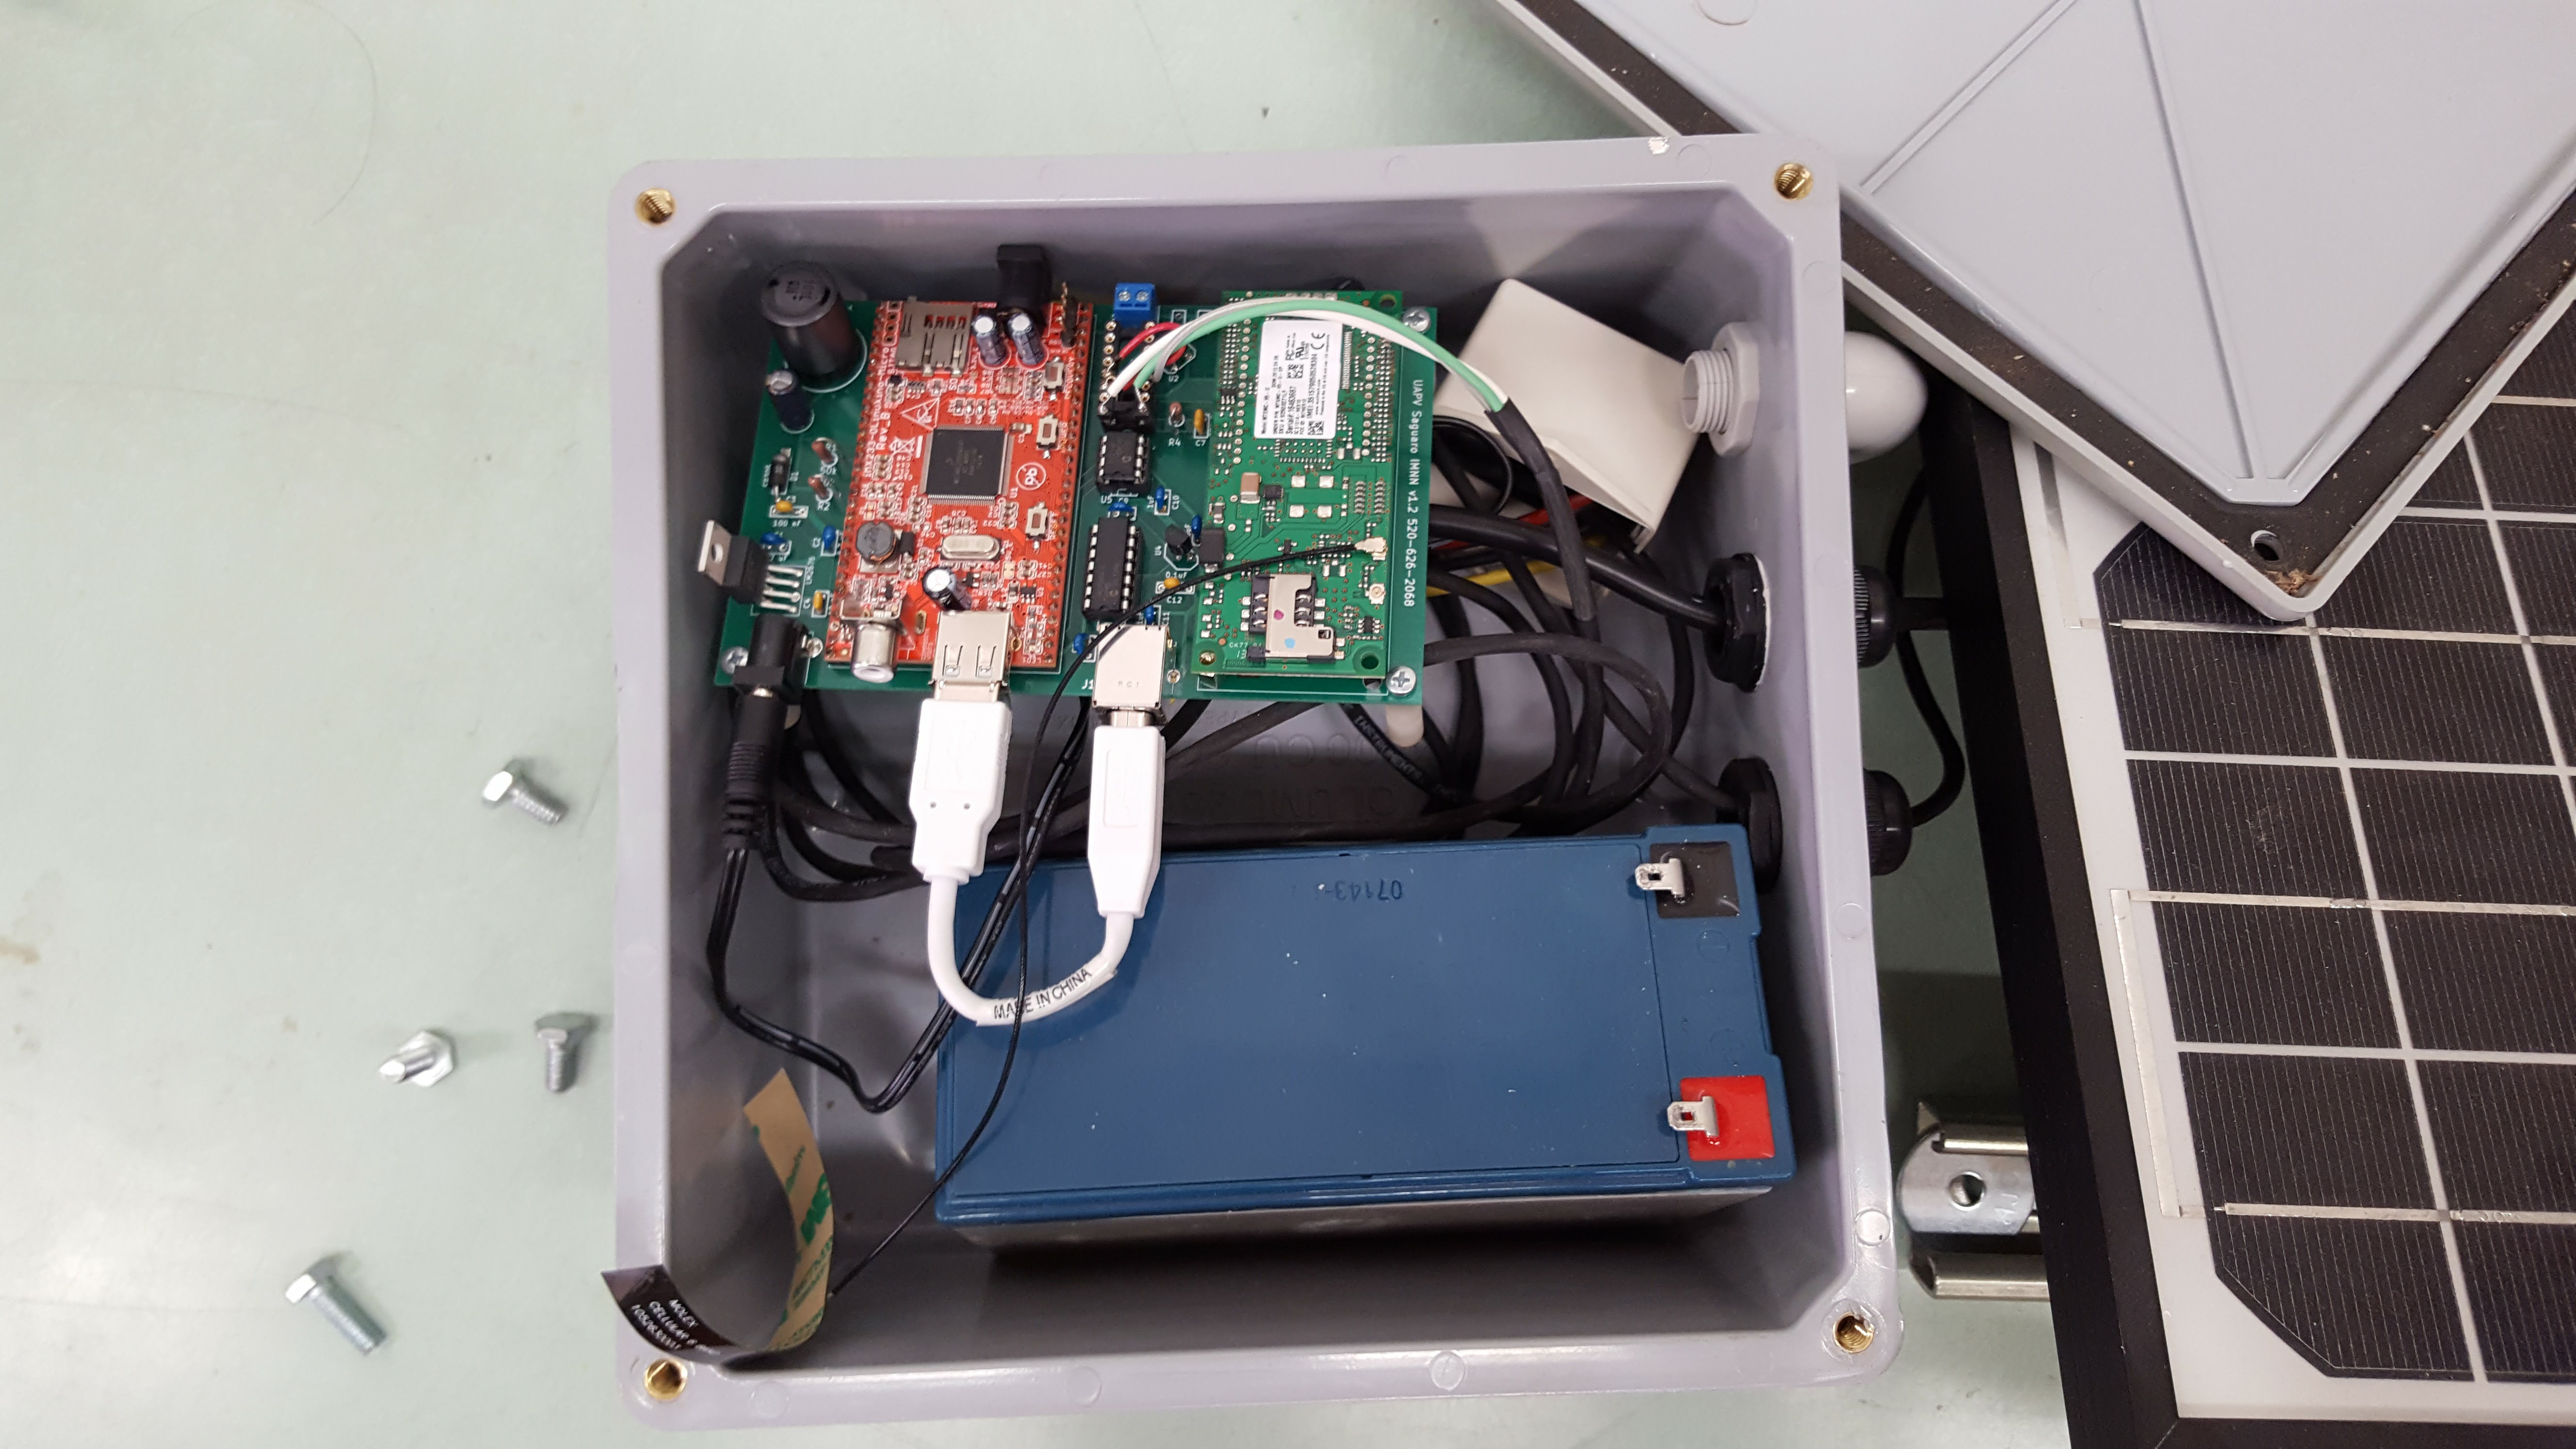
\includegraphics[width=0.65\textwidth]{../dissertation/figs/sensor_interior.jpg}}
\hspace{0.1em}
\subfloat{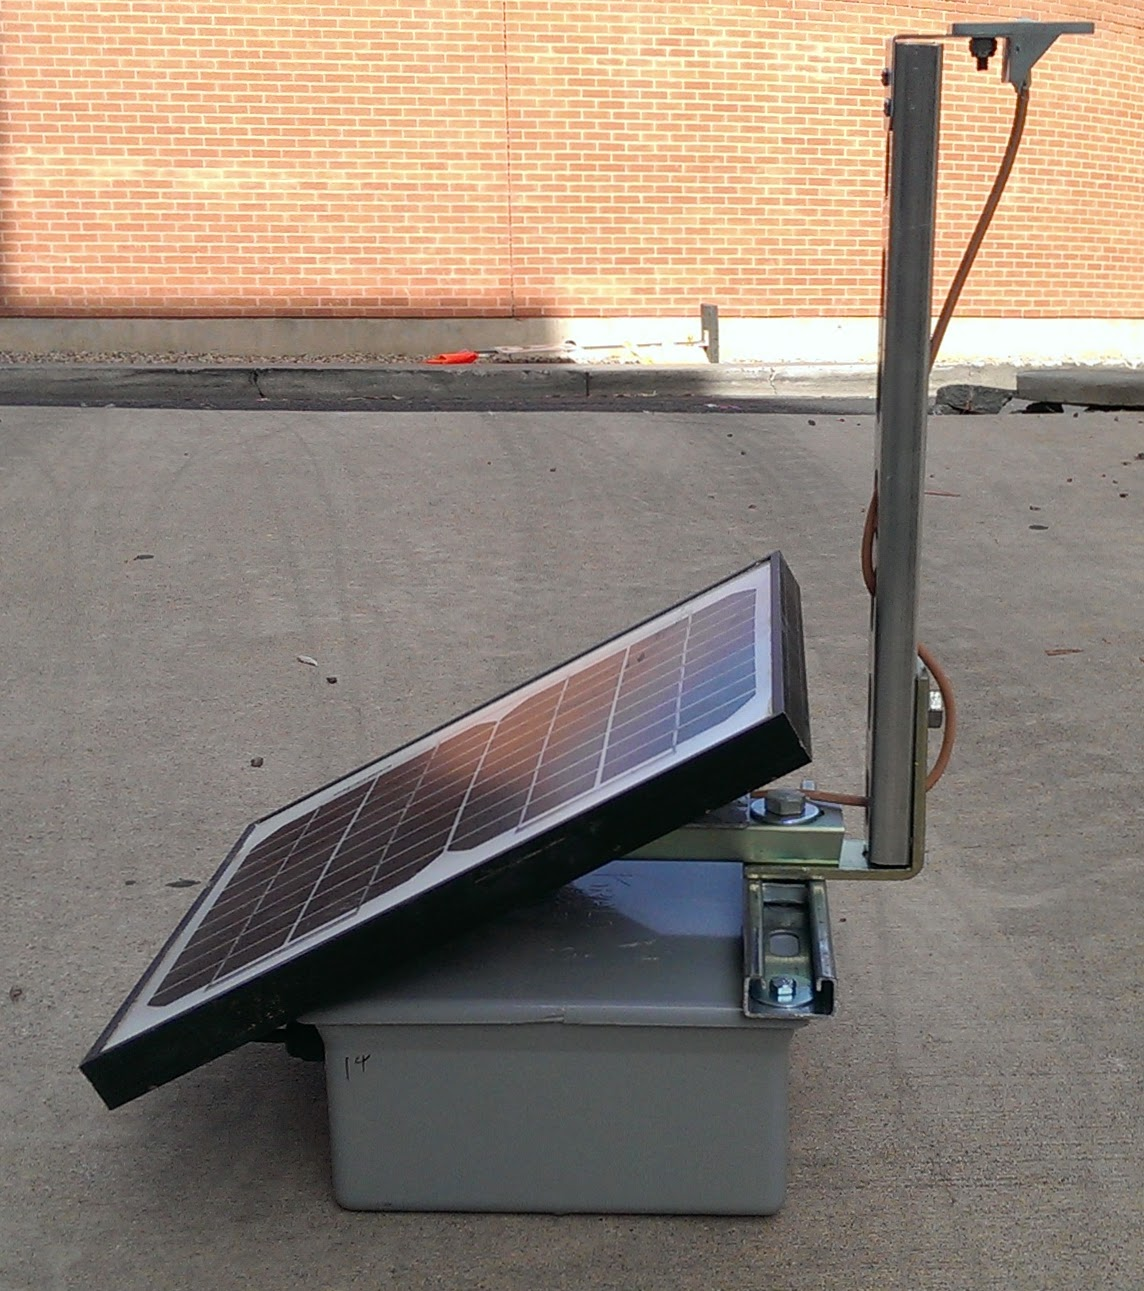
\includegraphics[width=0.325\textwidth]{../dissertation/figs/sensor_outside.jpg}}
\caption{Photos of the interior and exterior of the custom sensors
  used in the irradiance network.}
\label{fig:sensor}
\end{figure}

We iterated through a number of designs before arriving at the design
shown in \cref{fig:sensor}.
The sensors utilize a small Linux computer to collect the data from a
photodiode sensor, a solar panel and battery for power, and a cell
modem to send the data to a central server every minute.
These sensors provided high quality data from April to July 2014
before a flaw with the installation method killed many of the sensors.

With the help of Technicians for Sustainability, we also receive data
from rooftop PV systems every five minutes.
A map of the sensor network is shown in \cref{fig:networkmap}.

\begin{figure}[h]
\centering
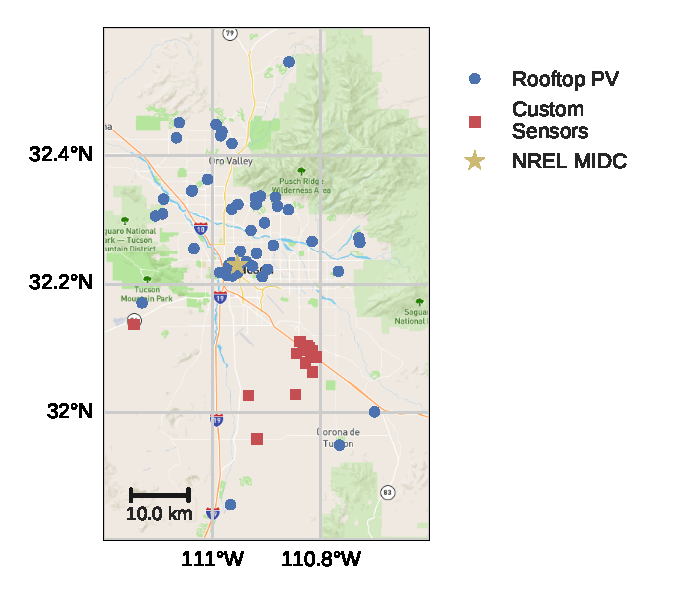
\includegraphics[width=0.5\textwidth]{../dissertation/figs/map.pdf}
\caption[Map of sensor locations]{Map of Tucson, AZ, indicating the
  locations of custom and rooftop PV sensors. The NREL MIDC star
  refers to the calibrated and maintained irradiance sensor located at
  the University of Arizona.}
\label{fig:networkmap}
\end{figure}


\section{Irradiance Network Forecasts}
\begin{figure}[h]
\centering
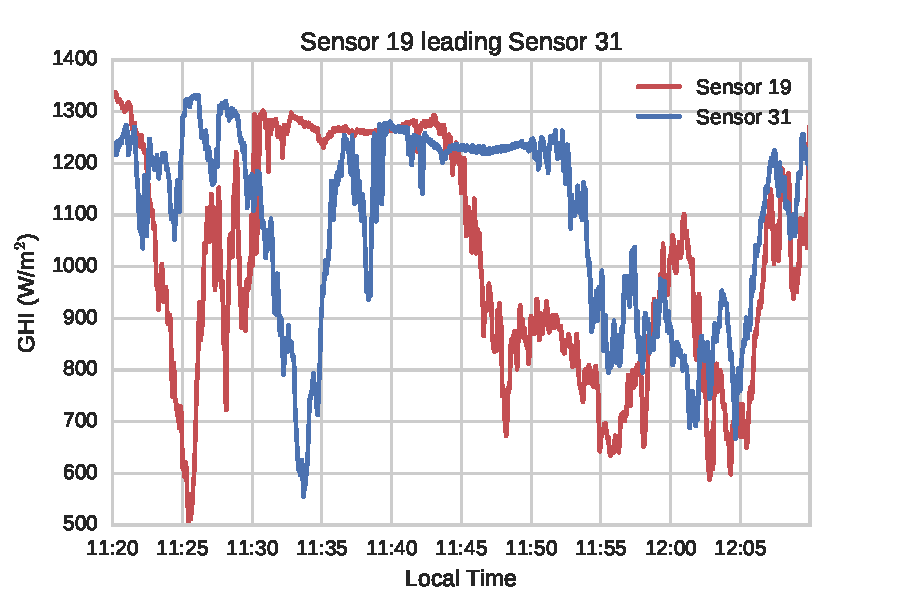
\includegraphics[width=0.5\textwidth]{../dissertation/figs/leading_sens.pdf}
\caption{An example of the output of sensor 19 (red) predicting what
  the output of the upstream sensor 31 (blue) in roughly 8
  minutes.}
\label{fig:leading}
\end{figure}

The basic idea behind the irradiance network forecasts is that a drop
in the GHI recorded by one sensor may predict a future drop in GHI at
another sensor downstream as illustrated in \cref{fig:leading}.
To make the forecasts based on the irradiance monitoring network, we
first interpolate data from the sensors to produce a kind of cloud
map.
This map could then be translated based on some derived cloud-motion
vector to generate a forecast.

We have shown that a forecast made in this way outperforms a
persistence model that incorporates the diurnal cycle of GHI.
We also found that spatial or time averaging can produce skillful
forecasts which led to an in depth study of how one might present
error metrics in a Taylor diagram to determine the best forecast.
Errors for these forecasts are shown in \cref{fig:bullshitplot}.

\section{Optimal Interpolation of Network Data and Satellite Images}
Optimal interpolation (OI) is a Bayesian technique to combine the two
pieces of information accounting for the relative error between them.
We were able to apply OI to correct satellite estimated GHI with data
from the ground network even at locations in the image without nearby
sensors.
An example of the improvement due to OI is shown in \cref{fig:satoi}
and the improvement in RMSE over 3 months is shown in \cref{fig:bullshitplot}.

\begin{figure}[h]
\centering
\subfloat{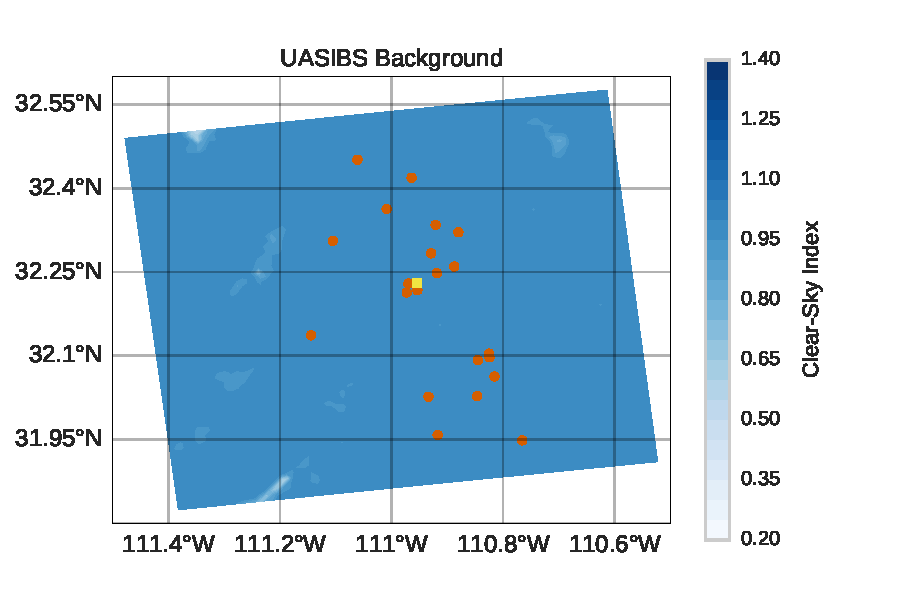
\includegraphics[width=0.5\textwidth]{figs/uasibs_bck_ex.pdf}}
\subfloat{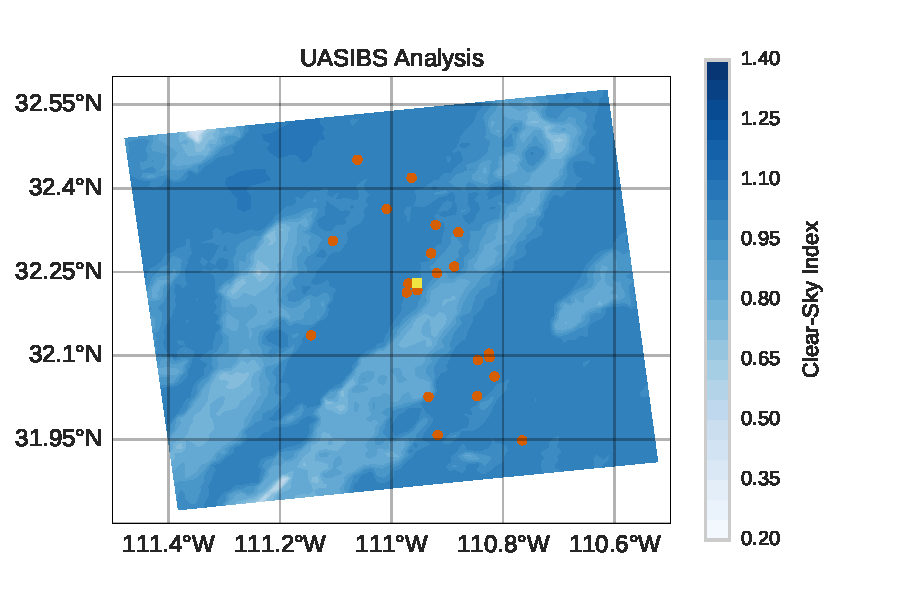
\includegraphics[width=0.5\textwidth]{figs/uasibs_anl_ex.pdf}}
\caption{An example of the satellite estimate clear-sky index (GHI /
  GHI$_{clear}$) before (left) and after (right) OI. The initial
  satellite estimate failed to produce enough clouds but OI corrects
  this.}
\label{fig:satoi}
\end{figure}


These nowcasts of GHI using a satellite image provide broad areal
coverage which is useful for estimating the generation of distributed,
rooftop PV systems and for resource assessment.
When combined with a cloud advection model, OI can be extended to the
well known Kalman filter and one can continuously incorporate new data
into the forecast.

\section{Conclusion}
This dissertation explores the use of an irradiance monitoring network
to improve solar irradiance forecasts that help electric utilities use
more solar power.
First, an irradiance monitoring network was designed and deployed \citep{Lorenzo2014}.
Then, data from this network was used directly to produce irradiance
forecasts that show an average of 20\% skill over a high-quality
persistence method \citep{Lorenzo2015c}.
Finally, the data from the network was used to correct satellite
derived irradiance images that will be the basis of forecasts in the
future \citep{Lorenzo2017}.
Future work in the group will continue to solidify the dashed lines in
\cref{fig:bullshitplot} to produce the best irradiance forecasts at
all time horizons.

\bibliographystyle{../dissertation/ieeetran}
\bibliography{../dissertation/bibliography}

\end{document}

%%% Local Variables:
%%% mode: latex
%%% TeX-master: t
%%% End:
